\begin{figure*}[tb]
	\noindent\begin{minipage}[b]{\columnwidth}
		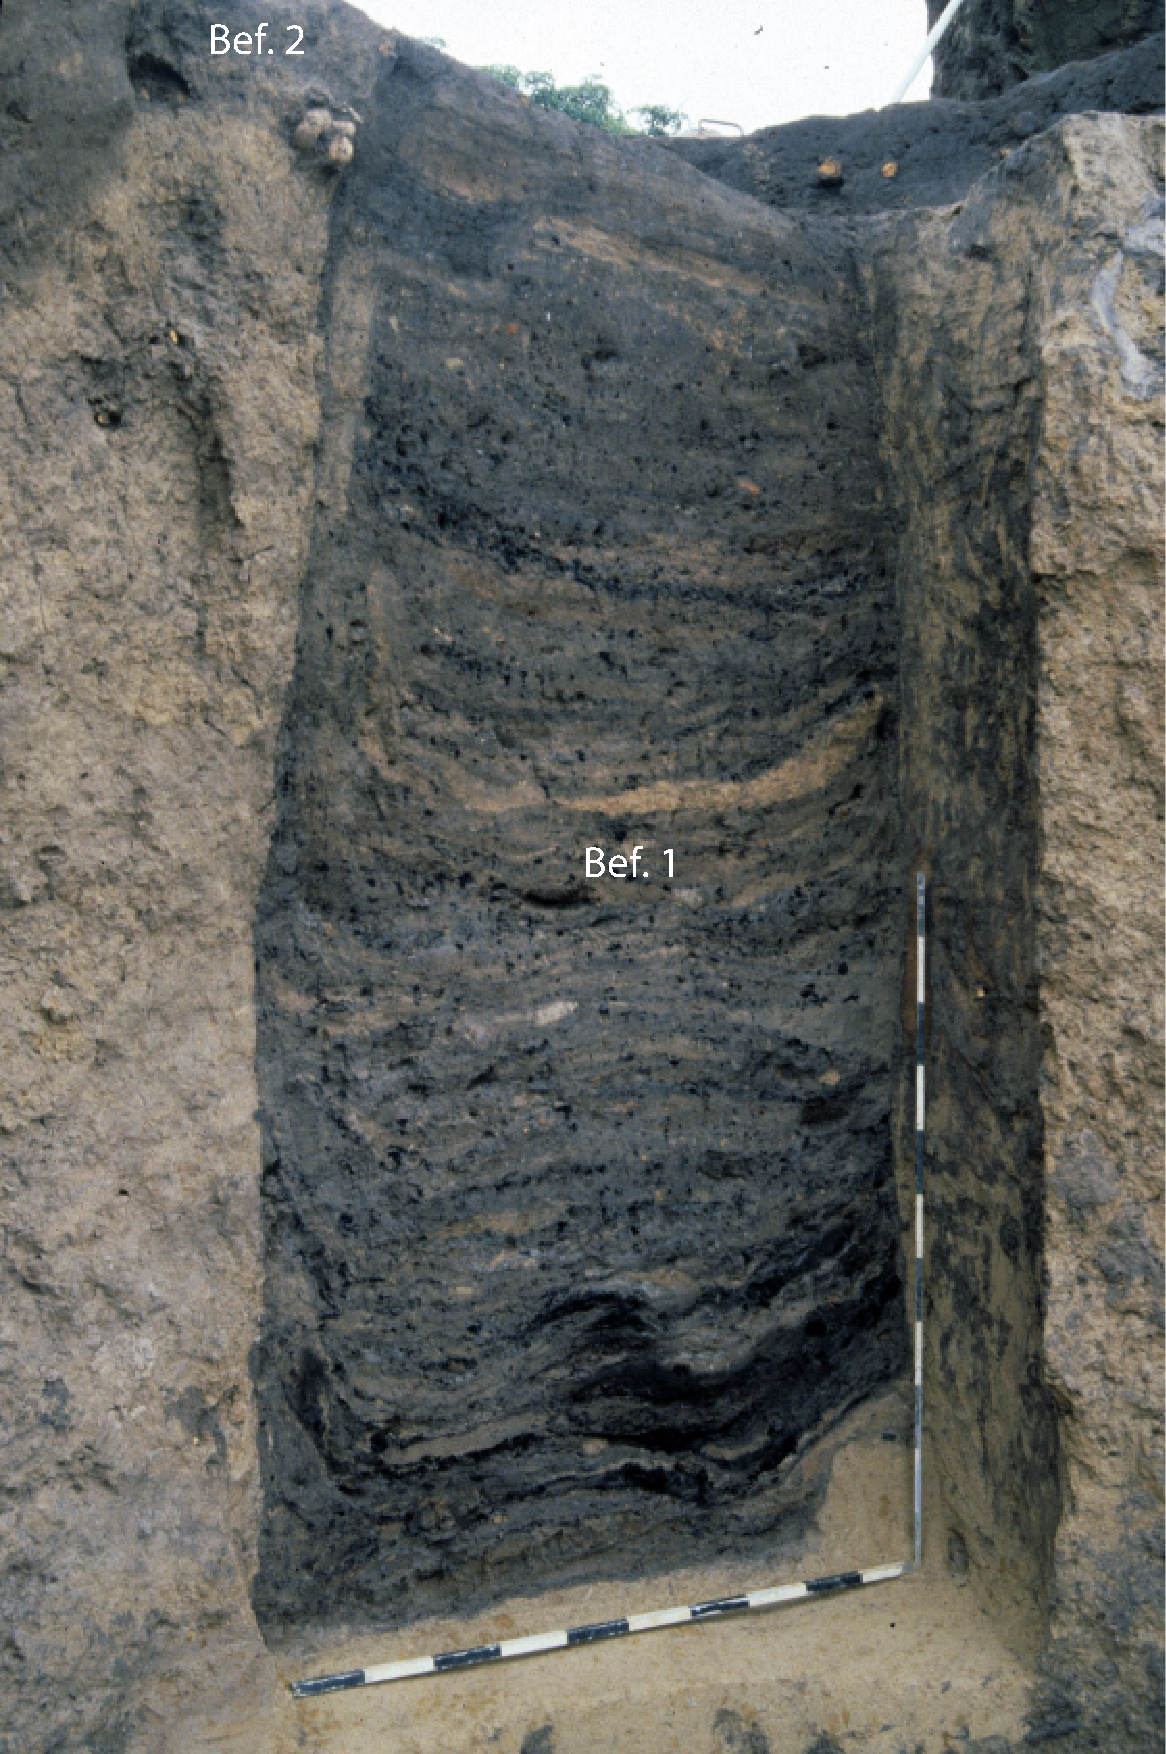
\includegraphics[width=\columnwidth]{fig/MLB85-2_Profil_E85-031-4.pdf}
		\captionof{figure}{MLB~85/2: Zurückverlegtes und geputztes Profil (Foto: M. K. H. Eggert, 1985).\label{fig:MLB85-2_Prof_geputzt}}
	\end{minipage}\hfill
	\noindent\begin{minipage}[b]{\columnwidth}
		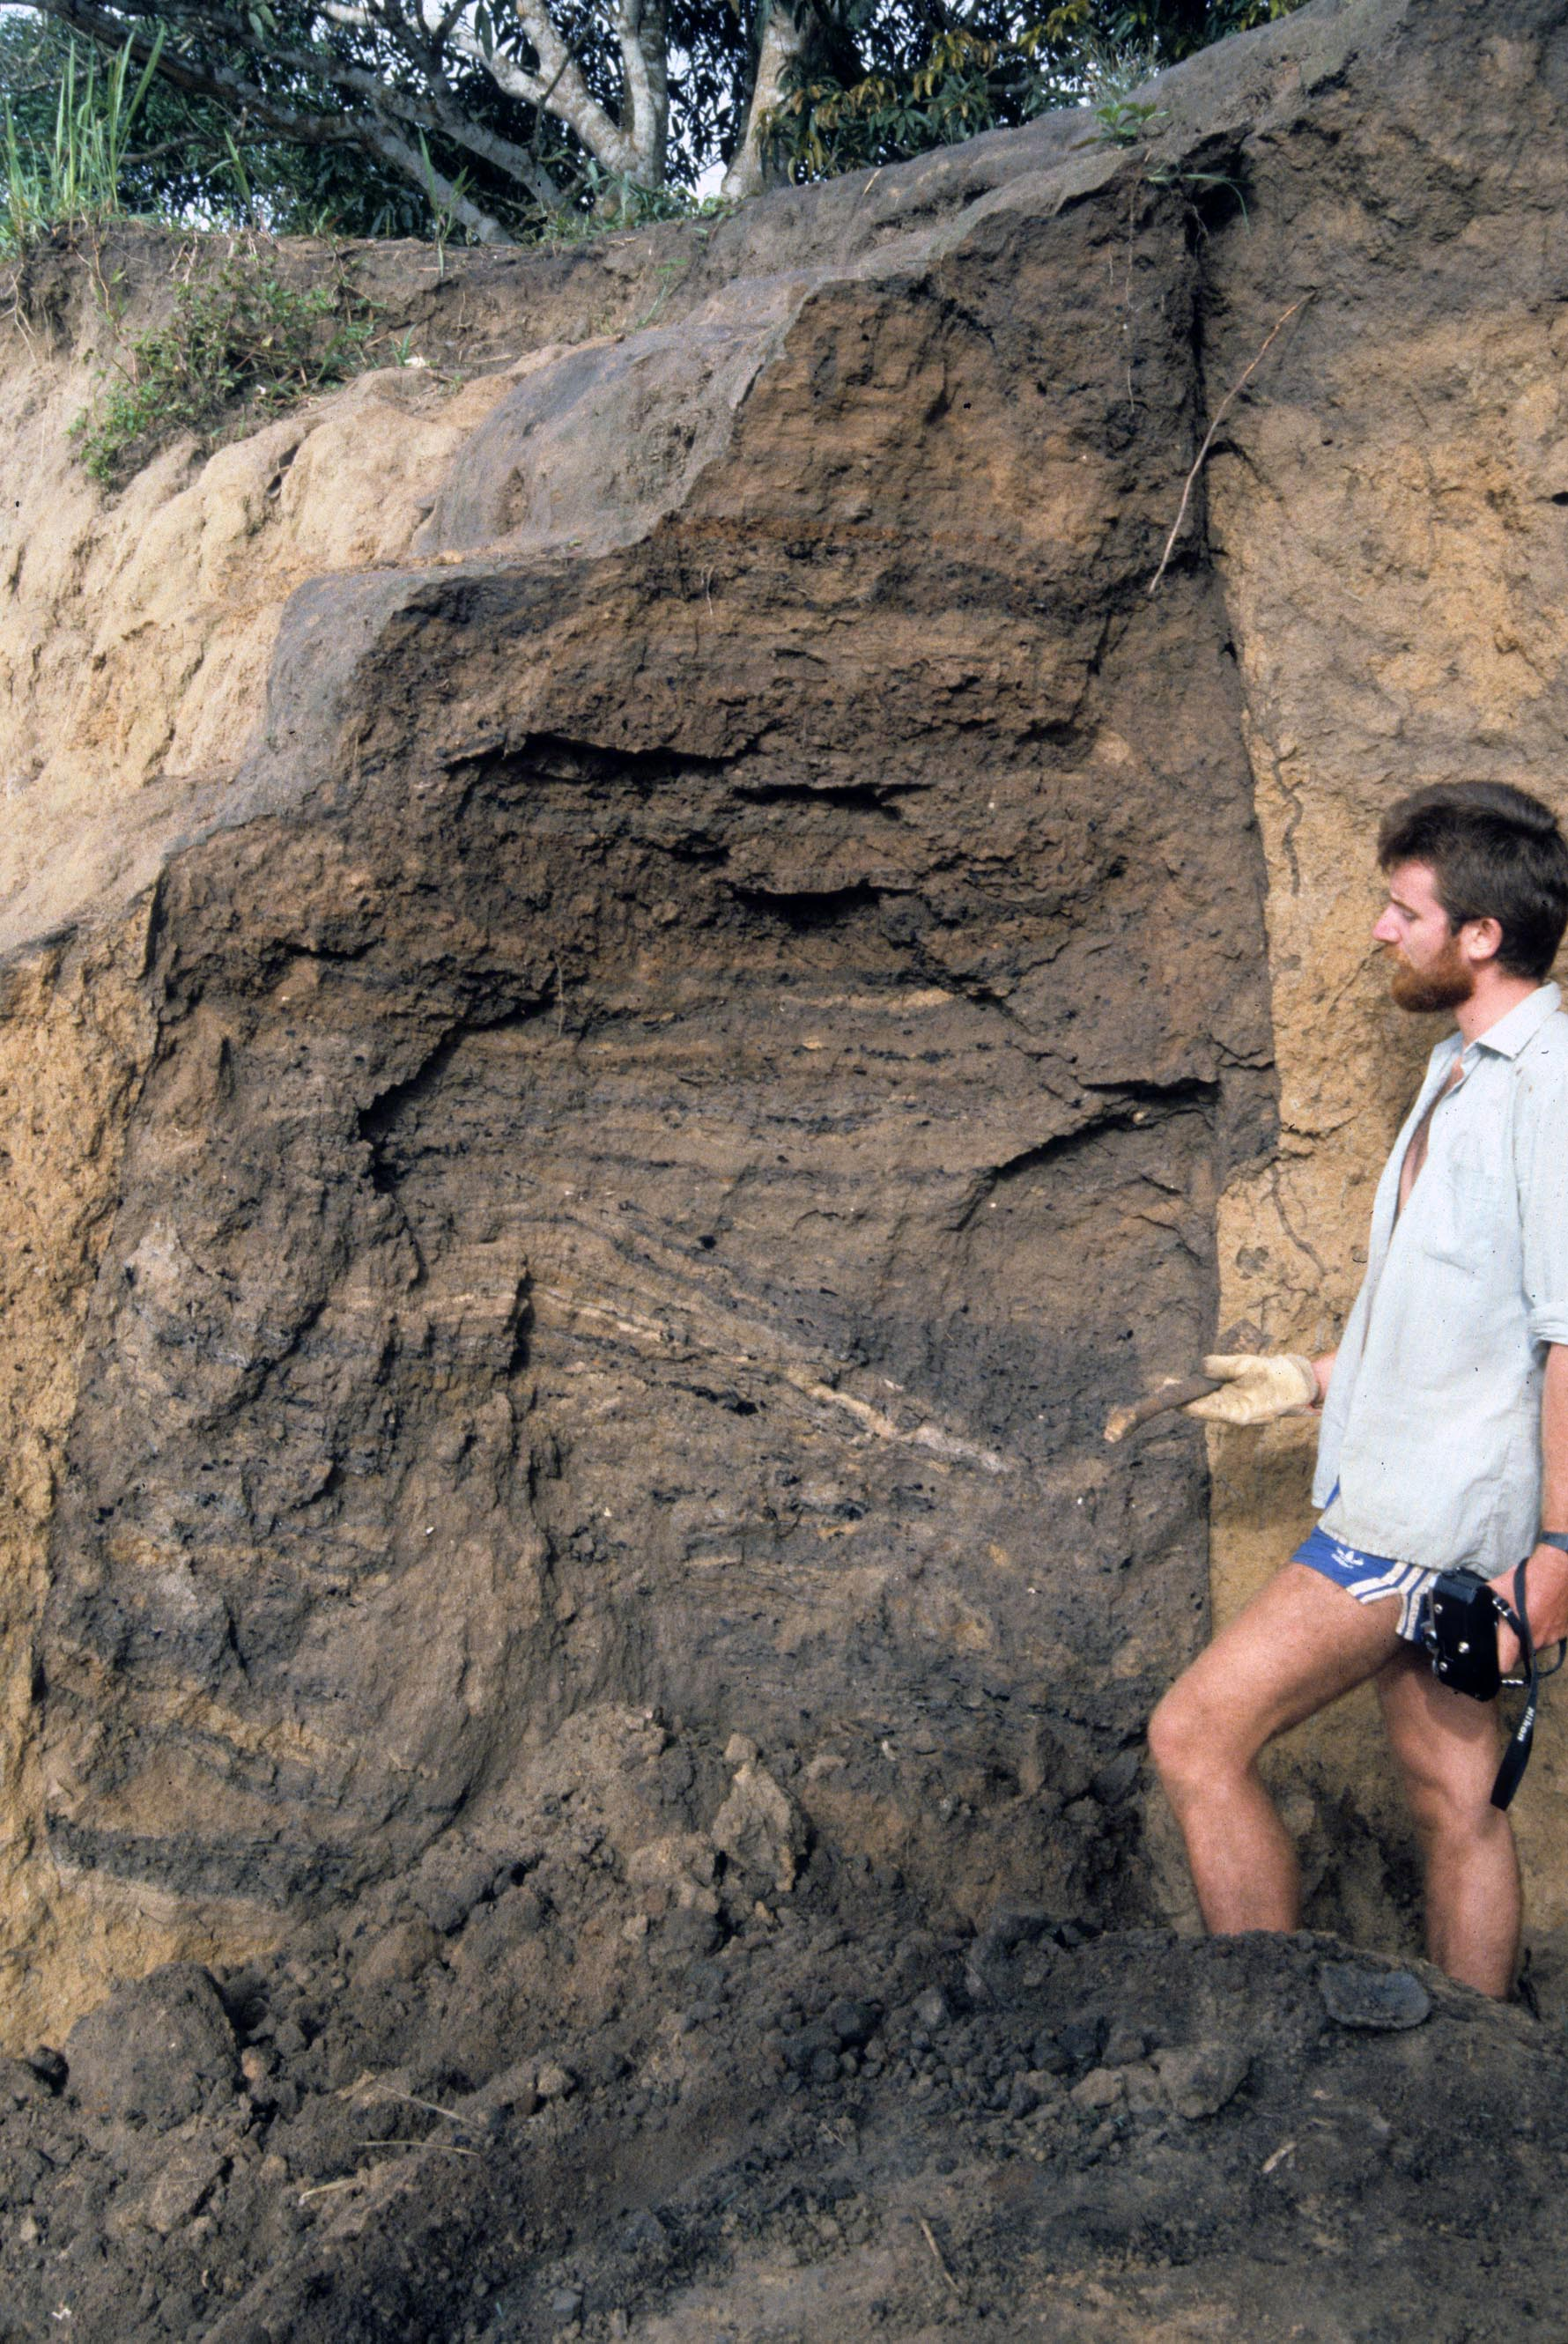
\includegraphics[width=\columnwidth]{fig/MLB85-103_E85-030-27.jpg}
		\captionof{figure}{MLB 85/103: Teilweise freierodierte Grube in der Uferböschung des Lua in Maluba (Foto: M. K. H. Eggert, 1985).\label{fig:MLB85-103_ProfilFoto}}
	\end{minipage}
\end{figure*}

\section*{\begin{tabular*}{\linewidth}{@{}l @{\extracolsep{\fill}} r@{}}
Nr.~4 & MLB~85/2\\
\end{tabular*} 
}

\textsf{\textbf{Maluba (Lua; Fpl.~230)}}

\vspace{1em}

\noindent\begin{tabular}{@{}rl@{}}
\textbf{Feldarbeit:} & \begin{tabular}[t]{@{}l@{}}\textbf{05.09.--06.09.1985 (C. Kanimba}\\ \textbf{Misago/H.-P. Wotzka)}\end{tabular} \\ 
\textbf{Abb.:} & \textbf{\ref{fig:MLB85-2_Prof_geputzt}} \\
\textbf{Lit.:} & \textbf{--} \\ 
\end{tabular}

\paragraph{Grabung und Befunde}\hspace{-.5em}|\hspace{.5em}%
Die 2,55\,m tiefe, kasten- bis leicht trapezförmige Grube zeichnete sich im Uferprofil durch eine scharf begrenzte dunkle Verfüllung ab. Sie hat einen Durchmesser von etwa 1,1~m, eine horizontale Sohle und vertikale bis leicht steilschräg überkippte Wandungen. Im unteren Teil weist sie eine horizontale, stark holzkohlehaltige, feine Bänderung auf. Direkt neben der Grube fand sich eine Körperbestattung, aus welcher kurz vor der Grabung bereits Skelettteile gefallen waren. Nach dem Profilputz ragten noch Knochen der unteren Extremitäten -- Unterschenkel und Fußwurzel sowie Teile der Mittelfußknochen, aber keine Zehen -- aus dem Profil (Abb.~\ref{fig:MLB85-2_Prof_geputzt}). Das Grab durchschneidet eine rot verziegelte \textit{Plattform} oder Feuerstelle. 

Im ersten Planum, das etwa 0,3\,m unter der rezenten Oberfläche lag, waren Grube und Bestattung deutlich voneinander unterscheidbar, ohne dass das zeitliche Verhältnis beider Befunde eindeutig war. Die von der Bestattung durchschnittene, gebänderte Lage angeziegelten Materials war über der Grube nicht erkennbar. Das Grab ist durchgehend etwa 0,4\,m breit. Seine dunkle Verfüllung ist stark mit hellen Sandflecken durchsetzt, während die Verfüllung der Grube homogen dunkelbraun ist und sich deutlich vom hellen anstehenden Sand absetzt.

Im Profil ist eine sehr fein laminierte Wechselschichtung von dunklen und hellen Lagen innerhalb der Grube erkennbar.\footnote{Die feine Wechselschichtung zusammen mit den scharfen Befundgrenzen kann als ein Indiz für ein junges Alter des Befundes gewertet werden. Die älteren, Keramik des Batalimo-Maluba-Stils enthaltenden und in die Jahrhunderte um die Zeitenwende datierten Gruben MLB~85/1-3-1 und MLB~85/1-3-2 (Kat.-Nr.~1--2) zeigen weder eine fein laminierte Schichtung noch scharfe Befundgrenzen.} Am zweiten Tag der Grabung stürzte aufgrund von starkem Regen das Profil teilweise ein. Die Grabung wurde danach nicht mehr weitergeführt.\footnote{Im eingestürzten Zustand konnte noch beobachtet werden, dass das Grab die Grube teilweise schneidet und somit stratigrafisch jünger ist. Die Bestattung ist bei dem Abrutschen des Materials  weiter herausgebrochen.}

\paragraph{Funde}\hspace{-.5em}|\hspace{.5em}%
Es lagen keine Funde aus dem Befund MLB~85/2 zur Auswertung vor.\footnote{Auf einigen der verfügbaren Situationsfotos, die währen der Anlage des ersten Abtrages gemacht wurden, ist zu sehen, dass Funde abgesammelt wurden und der Ausgräber C. Kanimba Misago neben sich ein Körbchen mit Scherben liegen hat. Was mit diesen Funden passiert ist und warum sie nicht beim restlichen Fundgut verblieben sind, lässt aus der vorhandenen Aktenlage nicht mehr rekonstruieren.} Da auch kein Probenmaterial für Radiokohlenstoffdatierungen vorliegt, ist eine Datierung des Befundes nicht möglich.